\documentclass[conference]{IEEEtran}
\IEEEoverridecommandlockouts
\usepackage{tabularx}
\usepackage{booktabs}
\usepackage{cite}
\usepackage{amsmath,amssymb,amsfonts}
\usepackage{algorithmic}
\usepackage{graphicx}
\usepackage{textcomp}
\usepackage{xcolor}
\usepackage{newtxtext,newtxmath}
\usepackage{xurl}

\begin{document}

\title{Comparing Critic and User Movie Reviews Using Data Mining}

\author{\IEEEauthorblockN{1\textsuperscript{st} Brady Lauritsen}
  \IEEEauthorblockA{\textit{Computer Science} \\
    \textit{University of Nebraska-Lincoln}\\
    Lincoln, NE, USA}
  \and
  \IEEEauthorblockN{2\textsuperscript{nd} Sagun Karki}
  \IEEEauthorblockA{\textit{Computer Science \& Data Science} \\
    \textit{University of Nebraska-Lincoln}\\
    Lincoln, NE, USA}
  \and
  \IEEEauthorblockN{3\textsuperscript{rd} Harrison Johs}
  \IEEEauthorblockA{\textit{Computer Science} \\
    \textit{University of Nebraska-Lincoln}\\
    Lincoln, NE, USA}
  \and
  \IEEEauthorblockN{4\textsuperscript{th} Max Buettenback}
  \IEEEauthorblockA{\textit{Computer Science} \\
    \textit{University of Nebraska-Lincoln}\\
    Lincoln, NE, USA}
}

\maketitle

\begin{abstract}
  This project investigates the discrepancy between professional critic reviews and general audience ratings. Using data from Rotten Tomatoes and Letterboxd, we integrated over 800,000 records to analyze patterns in film evaluation. By performing preprocessing, association mining, sentiment analysis, and predictive modeling, we determine how well critic consensus predicts audience sentiment. Our finalized Random Forest model achieved a highly successful R-squared value of 0.7831, proving that professional critical consensus remains a powerful leading indicator of community taste.
\end{abstract}

\begin{IEEEkeywords}
  data mining, sentiment analysis, professional reviews, audience ratings, predictive modeling
\end{IEEEkeywords}

\section{Introduction}
The difference between professional critic reviews and general audience reviews has long been a topic of discussion in the film industry. Critics often evaluate films based on technical quality, artistic merit, and narrative structure, while general audiences may prioritize entertainment value and personal enjoyment. This project explores whether the digital democratization of criticism on platforms like Letterboxd has created a total divide, or if critics still serve as an anchor for general taste.

\section{Objectives}
\begin{itemize}
  \item \textbf{Objective 1 -- Data Preprocessing:} Clean and merge datasets into a 806,405-record unified file.
  \item \textbf{Objective 2 -- Association Mining:} Discover frequent patterns and hidden rules within the dataset to identify specific conditions (such as genre combinations or release eras) under which critic and audience evaluations systematically diverge.
  \item \textbf{Objective 3 -- Sentiment Analysis:} Analyze review text to compare emotional tone and predictive granularity.
  \item \textbf{Objective 4 -- Predictive Modeling:} Develop ensemble models to forecast user ratings based on critic metadata.
\end{itemize}

\section{Datasets}

\subsection{Dataset 1: Rotten Tomatoes}
\begin{itemize}
  \item \textbf{Source:} Kaggle \cite{leone2020rotten}
  \item \textbf{Size:} 17,000+ movies and 1M+ critic reviews.
  \item \textbf{Scope:} Data scraped as of October 2020.
\end{itemize}

\begin{table}[htbp]
  \caption{Rotten Tomatoes Key Attributes}
  \begin{center}
    \begin{tabularx}{\columnwidth}{|l|l|X|}
      \hline
      \textbf{Attribute}  & \textbf{Data Type} & \textbf{Description}               \\ \hline
      movie\_title        & Nominal            & The official title of the film.    \\ \hline
      genres              & Nominal            & Categorical genre tags.            \\ \hline
      tomatometer\_rating & Ratio              & Professional critic score (0-100). \\ \hline
      review\_content     & Nominal            & Raw text of the critic review.     \\ \hline
      release\_year       & Interval           & The year the movie was released.   \\ \hline
    \end{tabularx}
    \label{tab1}
  \end{center}
\end{table}

\subsection{Dataset 2: Letterboxd}
\begin{itemize}
  \item \textbf{Source:} Kaggle \cite{letterboxd2020}
  \item \textbf{Size:} Approximately 2.5 million user ratings.
  \item \textbf{Scope:} User-submitted ratings on a 0.5--5 star scale.
\end{itemize}

\begin{table}[htbp]
  \caption{Letterboxd Key Attributes}
  \begin{center}
    \begin{tabularx}{\columnwidth}{|l|l|X|}
      \hline
      \textbf{Attribute} & \textbf{Data Type} & \textbf{Description}                 \\ \hline
      movie\_title       & Nominal            & The title used for dataset matching. \\ \hline
      rating\_val        & Ordinal            & User score from 0.5 to 5.0.          \\ \hline
      user\_id           & Nominal            & Unique identifier for the user.      \\ \hline
      year\_released     & Interval           & Release year for matching purposes.  \\ \hline
    \end{tabularx}
    \label{tab2}
  \end{center}
\end{table}

\section{Data Processing (Harrison Johs)}

\section{Methods}
\subsection{Association Mining (Max Buettenback)}

\subsection{Sentiment Analysis (Sagun Karki)}


\subsection{Predictive Modeling (Brady Lauritsen)}
We implemented Linear Regression and Random Forest models to forecast community ratings. The Random Forest Regressor utilized 200 estimators and a max depth of 10. By integrating the Tomatometer consensus and release year, we were able to significantly outperform the linear baseline.

\section{Experimental Results}
The evaluation demonstrates that our ensemble model is highly effective, capturing 78.31\% of the variance in audience taste.

\begin{table}[htbp]
  \caption{Model Performance Comparison}
  \begin{center}
    \begin{tabular}{|l|c|c|c|}
      \hline
      \textbf{Model}         & \textbf{MSE}   & \textbf{RMSE} & \textbf{R-Squared} \\ \hline
      Linear Regression      & 53.53          & 7.32          & 0.7077             \\ \hline
      \textbf{Random Forest} & \textbf{39.72} & \textbf{6.30} & \textbf{0.7831}    \\ \hline
    \end{tabular}
  \end{center}
\end{table}

\begin{figure}[htbp]
  \centerline{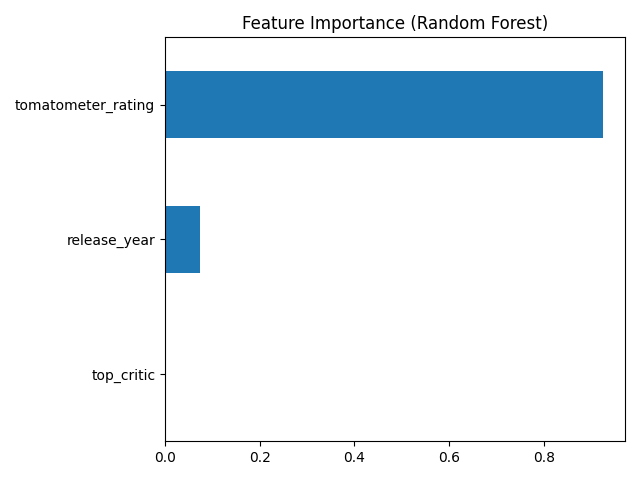
\includegraphics[width=\columnwidth]{Figures/feature_importance.png}}
  \caption{Feature Importance analysis showing the dominance of the Tomatometer.}
  \label{fig_importance}
\end{figure}

As shown in Figure \ref{fig_importance}, the Tomatometer consensus is the primary driver of the model, accounting for 92.8\% of the decision-making importance. This confirms that community sentiment is heavily anchored to the professional consensus. The Release Year (6.3\%) also proved significant, suggesting shifts in rating behaviors across different eras.

\begin{figure}[htbp]
  \centerline{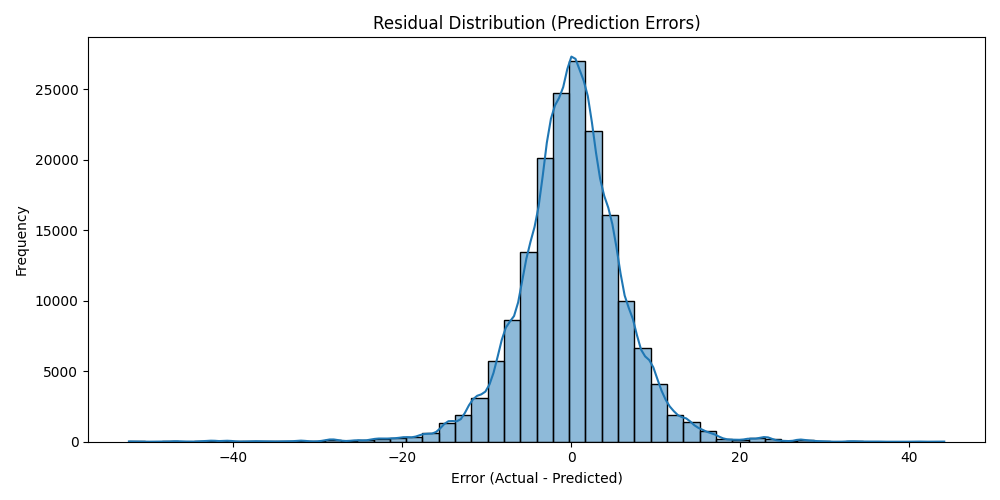
\includegraphics[width=\columnwidth]{Figures/residuals.png}}
  \caption{Residual distribution confirming an unbiased predictive model.}
  \label{fig_residuals}
\end{figure}

Furthermore, the residual distribution in Figure \ref{fig_residuals} follows a symmetric bell curve centered at zero. This proves the model is statistically objective and does not systematically over-predict or under-predict ratings across the 578,752 records used in the finalized training set.

\section{Logistics}
The team met virtually every Wednesday at 3:00 PM CST to coordinate repository merges, troubleshoot preprocessing conflicts, and synchronize experimental findings.

\section{Team Contributions}
\begin{itemize}
  \item \textbf{Brady Lauritsen:} Lead for Predictive Modeling; implemented Random Forest and performed model evaluation.
  \item \textbf{Sagun Karki:} Lead for Sentiment Analysis; analyzed emotional tone and its relationship to numerical scores.
  \item \textbf{Harrison Johs:} Lead for Data Preprocessing; integrated the large datasets and performed cleaning.
  \item \textbf{Max Buettenback:} Lead for Association Mining; identified frequent patterns and rule-based relationships across film genres and eras.
\end{itemize}

\section{Conclusion}
This project successfully quantified the relationship between critics and audiences.

\bibliographystyle{IEEEtran}
\bibliography{references}
\end{document}